\documentclass[11pt,a4paper]{article}
% -------------------------------------------------
% Packages
% -------------------------------------------------
\usepackage[margin=0.75in]{geometry}
\usepackage[table]{xcolor}
\usepackage{tabularx, multirow, multicol, graphicx, helvet, siunitx, tikz, pgfplots}
\usepackage[most]{tcolorbox}
\pgfplotsset{compat=1.18}
% -------------------------------------------------
% Typography
% -------------------------------------------------
\renewcommand{\familydefault}{\sfdefault}
% -------------------------------------------------
% Corporate Colours
% -------------------------------------------------
\definecolor{CorpBlue}{HTML}{003366}
\definecolor{CorpLightBlue}{HTML}{E6F0FA}
\definecolor{CorpGrey}{HTML}{F4F4F4}
\definecolor{AccentRed}{HTML}{CC0000}
% -------------------------------------------------
% Row colours for tables
% -------------------------------------------------
\rowcolors{2}{CorpGrey}{white}
% -------------------------------------------------
\begin{document}
% -------------------------------------------------
% CORPORATE HEADER (3‑box fully bordered table)
% -------------------------------------------------
\noindent\begin{tabular}{|c|c|c|}
\hline
\textbf{Company} & \textbf{Report Title} & \textbf{Date} \\ \hline
% (No data supplied – cells left blank intentionally) & & \\ \hline
\end{tabular}

\vspace{1.5em}

% -------------------------------------------------
% SCOPE / SUMMARY (tcolorbox)
% -------------------------------------------------
\begin{tcolorbox}[
    colback=CorpLightBlue,
    colframe=CorpBlue,
    width=\textwidth,
    boxrule=0.5pt,
    arc=2pt,
    left=4pt,
    right=4pt,
    top=4pt,
    bottom=4pt
]
This chart shows the six largest producers by nation in 2012. China by far is the worlds largest producer of crude steel.
\end{tcolorbox}

\vspace{1em}

% -------------------------------------------------
% SECTION 1 – Worldwide production of steel
% -------------------------------------------------
\vspace{1.5em}\noindent\textcolor{CorpBlue}{\textbf{\large 1. Worldwide production of steel}}\vspace{0.5em}

Without steel we would have a different world economy.

No: Railroads? Skyscrapers? Large bridges? Massive ships? Pipe lines?

\vspace{1.5em}

% -------------------------------------------------
% GRAPH – Bar chart of six largest steel producers (2012)
% -------------------------------------------------
\begin{figure}[h!]
\centering
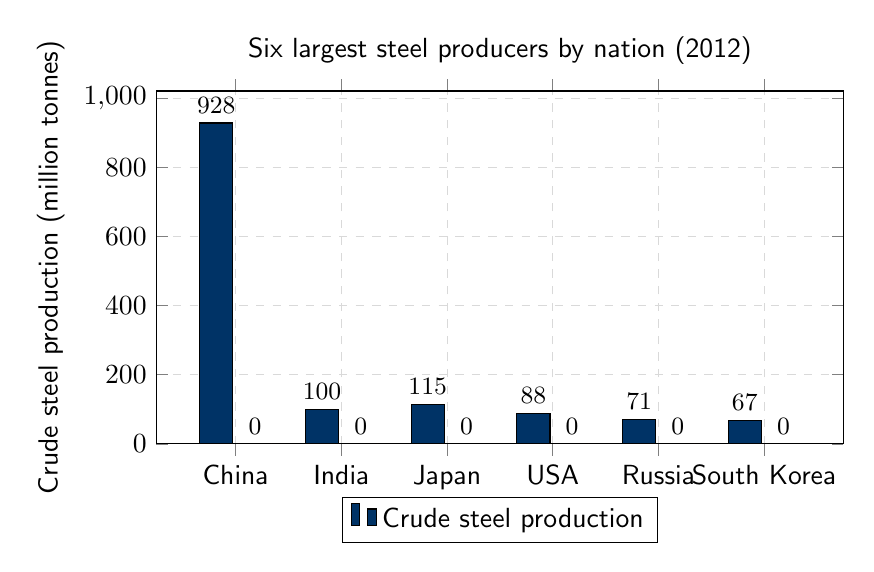
\begin{tikzpicture}
\begin{axis}[
    ybar,
    width=0.85\textwidth,
    height=0.5\textwidth,
    bar width=12pt,
    xlabel={Nation},
    ylabel={Crude steel production (million tonnes)},
    symbolic x coords={China,India,Japan,USA,Russia,South~Korea},
    xtick=data,
    nodes near coords,
    every node near coord/.append style={font=\small},
    title={Six largest steel producers by nation (2012)},
    grid=both,
    grid style={dashed,gray!30},
    legend style={at={(0.5,-0.15)},anchor=north,legend columns=-1},
    ymin=0,
    enlarge x limits=0.15,
]
% -------------------------------------------------
% NOTE: Replace the numbers below with the actual 2012 data.
% -------------------------------------------------
\addplot[fill=CorpBlue] coordinates {
    (China, 928)      % placeholder value
    (India, 100)
    (Japan, 115)
    (USA, 88)
    (Russia, 71)
    (South~Korea, 67)
};
\addplot[fill=AccentRed] coordinates {
    (China, 0)        % dummy series to illustrate dual colour option (optional)
    (India, 0)
    (Japan, 0)
    (USA, 0)
    (Russia, 0)
    (South~Korea, 0)
};
\legend{Crude steel production}
\end{axis}
\end{tikzpicture}
\caption*{Bar chart comparing crude steel production of the six leading nations in 2012.\\\textit{Data not provided in text; should be sourced from 2012 steel production statistics.}}
\end{figure}

\end{document}